\let\negmedspace\undefined
\let\negthickspace\undefined
\documentclass[journal]{IEEEtran}
\usepackage[a5paper, margin=10mm, onecolumn]{geometry}
%\usepackage{lmodern} % Ensure lmodern is loaded for pdflatex
\usepackage{tfrupee} % Include tfrupee package

\setlength{\headheight}{1cm} % Set the height of the header box
\setlength{\headsep}{0mm}     % Set the distance between the header box and the top of the text

\usepackage{gvv-book}
\usepackage{gvv}
\usepackage{cite}
\usepackage{amsmath,amssymb,amsfonts,amsthm}
\usepackage{algorithmic}
\usepackage{graphicx}
\usepackage{textcomp}
\usepackage{xcolor}
\usepackage{txfonts}
\usepackage{listings}
\usepackage{enumitem}
\usepackage{mathtools}
\usepackage{gensymb}
\usepackage{comment}
\usepackage[breaklinks=true]{hyperref}
\usepackage{tkz-euclide} 
\usepackage{listings}
\usepackage{gvv}                                        
\def\inputGnumericTable{}                                 
\usepackage[latin1]{inputenc}                                
\usepackage{color}                                            
\usepackage{array}                                            
\usepackage{longtable}                                       
\usepackage{calc}                                             
\usepackage{multirow}                                         
\usepackage{hhline}                                           
\usepackage{ifthen}                                           
\usepackage{lscape}
\usepackage{circuitikz}
\tikzstyle{block} = [rectangle, draw, fill=blue!20, 
    text width=4em, text centered, rounded corners, minimum height=3em]
\tikzstyle{sum} = [draw, fill=blue!10, circle, minimum size=1cm, node distance=1.5cm]
\tikzstyle{input} = [coordinate]
\tikzstyle{output} = [coordinate]


\begin{document}

\bibliographystyle{IEEEtran}
\vspace{3cm}

\title{2.8.39}
\author{EE25BTECH11049 - Sai Krishna Bakki}
 \maketitle
% \newpage
% \bigskip
{\let\newpage\relax\maketitle}

\renewcommand{\thefigure}{\theenumi}
\renewcommand{\thetable}{\theenumi}
\setlength{\intextsep}{10pt} % Space between text and floats


\numberwithin{equation}{enumi}
\numberwithin{figure}{enumi}
\renewcommand{\thetable}{\theenumi}

\textbf{Question}:\\
Find the angle between the lines whose direction cosines are given by the equations
 $l+m+n=0$, $l^2+m^2-n^2=0$. \\ 
\solution 
\section{Setting Up the Equations in Matrix Form}

We begin by representing the given system of equations using vectors and matrices. Let the direction cosines be represented by the column vector $\vec{x}$:
\begin{align}
\vec{x} = \myvec{l\\m\\n}
\end{align}
The three conditions on the direction cosines can be written in matrix form:
\begin{align}
 l + m + n = 0 \implies \vec{C}^T \vec{x} = 0, \vec{C} = \myvec{1\\1\\1}
 \end{align}
 \begin{align}
     l^2 + m^2 - n^2 = 0 \implies \vec{x}^T \vec{A} \vec{x} = 0, \vec{A} = \myvec{ 1 & 0 & 0 \\ 0 & 1 & 0 \\ 0 & 0 & -1 }
     \end{align}
     \begin{align}
     l^2 + m^2 + n^2 = 1 \implies \vec{x}^T \vec{I} \vec{x} = 1, \vec{I}=  \myvec{ 1 & 0 & 0 \\ 0 & 1 & 0 \\ 0 & 0 & 1 }
     \end{align}

\section{Solving for the Direction Cosine Vectors}

Our goal is to find the two vectors, $\vec{D}_1$ and $\vec{D}_2$, that satisfy these matrix equations.

\subsection{Finding the value of $n$ using Matrix Theory}
We can efficiently find the value of $n$ by subtracting the two quadratic form equations:
\begin{align}
\vec{x}^T \vec{I} \vec{x} - \vec{x}^T \vec{A} \vec{x} = 1 \implies \vec{x}^T (\vec{I} - \vec{A}) \vec{x} = 1
\end{align}
The matrix $(\vec{I} - \vec{A})$ is:
\begin{align}
\vec{I} - \vec{A} = \myvec{ 1 & 0 & 0 \\ 0 & 1 & 0 \\ 0 & 0 & 1 } -\myvec{ 1 & 0 & 0 \\ 0 & 1 & 0 \\ 0 & 0 & -1 } = \myvec{ 0 & 0 & 0 \\ 0 & 0 & 0 \\ 0 & 0 & 2 }
\end{align}
Substituting this back into the equation (0.5) gives:
\begin{align}
\myvec{ l & m & n } \myvec{ 0 & 0 & 0 \\ 0 & 0 & 0 \\ 0 & 0 & 2} \myvec{ l \\ m \\ n} = 1
\end{align}
\begin{align}
2n^2 = 1 \implies n = \pm \frac{1}{\sqrt{2}}
\end{align}

\subsection{Finding the values of $l$ and $m$}
Let's choose $n = -\frac{1}{\sqrt{2}}$. Substituting this into the remaining linear and normalization equations gives a system for $l$ and $m$:
\begin{align}
     \myvec{1&1&1}\myvec{l\\ m \\ \frac{-1}{\sqrt{2}}}=0 \implies l+m=\frac{1}{\sqrt{2}}
     \end{align}
     \begin{align}
     % l^2 + m^2 + \left(-\frac{1}{\sqrt{2}}\right)^2 = 1 \implies l^2 + m^2 = \frac{1}{2}
     \myvec{l &m &\frac{-1}{\sqrt{2}}}\myvec{ 1 & 0 & 0 \\ 0 & 1 & 0 \\ 0 & 0 & 1 }\myvec{l &m &\frac{-1}{\sqrt{2}}} \implies l^2 + m^2 = \frac{1}{2}
     \end{align}
     
Squaring the first part gives
\begin{align}
(l+m)^2 = \left(\frac{1}{\sqrt{2}}\right)^2 \implies l^2+2lm+m^2 = \frac{1}{2}
\end{align}

subsituting equation (0.10) in equation (0.11),we get
\begin{align}
    2lm=0
\end{align}
so we get l=0 and m=0,
\begin{align}
      l=0, m = \frac{1}{\sqrt{2}}\\
      m=0,l = \frac{1}{\sqrt{2}}
\end{align}


\subsection{Assembling the Direction Cosine Vectors}
Combining our results, the two direction cosine vectors are:
\begin{align}    
\vec{D}_1 = \myvec{ 0 \\ \frac{1}{\sqrt{2}} \\ \frac{-1}{\sqrt{2}} } \quad \text{and} \quad \vec{D}_2 = \myvec{ \frac{1}{\sqrt{2}} \\ 0 \\ \frac{-1}{\sqrt{2}}}
\end{align}


\section{Calculating the Angle using Matrix Theory}
The cosine of the angle $\theta$ between the lines is the dot product of their direction cosine vectors. Using matrix multiplication, this is 
\begin{align}
\cos \theta = \vec{D}_1^T \vec{D}_2\\ 
\cos \theta = \myvec{ 0 & \frac{1}{\sqrt{2}} & \frac{-1}{\sqrt{2}}} \myvec{ \frac{1}{\sqrt{2}} \\ 0 \\ \frac{-1}{\sqrt{2}} }
\end{align}


\begin{align}
\cos \theta = 0 + 0 + \frac{1}{2} = \frac{1}{2}
\end{align}
Therefore, the angle is:
\begin{align}
\theta = cos^{-1}\brak{\frac{1}{2}} = 60^{\circ} \quad \text{or} \quad \frac{\pi}{3} \text{ radians}
\end{align}
\newpage
 \begin{figure}
    \centering
    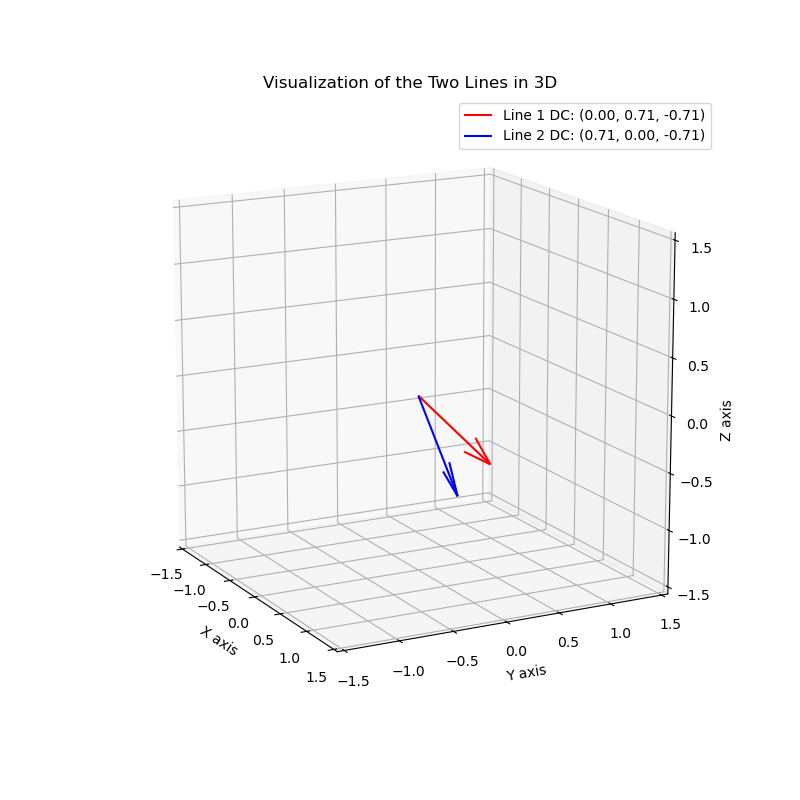
\includegraphics[width=0.9\columnwidth]{figs/Figure_1.png}
    \label{fig:placeholder}
\end{figure}
\end{document}
